% vim: set tabstop=4 shiftwidth=4

% Neovim setup:
% let g:vimtex_compiler_latexrun = {
%	\ 'build_dir' : '',
%	\ 'options' : [
%	\   '-verbose-cmds',
%	\   '-xelatex',
%	\   '-shell-escape',
%	\   '-interaction=nonstopmode',
%	\   '-synctex=1',
%	\   '-file-line-error',
%	\   '--latex-args="-shell-escape"',
%	\ ],
%	\}

% options:
% thesis=B bachelor's thesis
% thesis=M master's thesis
% czech thesis in Czech language
% english thesis in English language
% hidelinks remove colour boxes around hyperlinks

\documentclass[thesis=B,english]{FITthesis}[2019/12/23]
% TODO ✨remove from final build! ✨
\overfullrule=5pt

\usepackage[utf8]{inputenc} % LaTeX source encoded as UTF-8
% \usepackage[latin2]{inputenc} % LaTeX source encoded as ISO-8859-2
% \usepackage[cp1250]{inputenc} % LaTeX source encoded as Windows-1250

% \usepackage{subfig} %subfigures
% \usepackage{amsmath} %advanced maths
% \usepackage{amssymb} %additional math symbols

\usepackage{dirtree} %directory tree visualisation
\usepackage{xcolor}
\usepackage{blindtext}
\usepackage{footnote}
\usepackage{tabularx}
\usepackage{ragged2e}
\usepackage{booktabs}
\usepackage[numbers]{natbib}
\usepackage[htt]{hyphenat}
\usepackage{xparse,minted}
\usepackage{tikz}

\usetikzlibrary{
	shapes.multipart, arrows, positioning
}


% custom commands
\newcommand{\todo}[1]{\textcolor{red}{\textbf{[[#1]]}}}
\newcommand{\blind}[1][1]{\textcolor{gray}{\Blindtext[#1][1]}}
\newcommand{\citationNeeded}{\textcolor{red}{\textbf{[citation needed]}}}
\newcommand{\hackage}[1]{\texttt{#1}}
\newcommand{\hsSignature}[1]{\texttt{#1}}
\newcommand{\hsType}[1]{\texttt{#1}}
\newcommand{\hsIdent}[1]{\texttt{#1}}
\newcommand{\hsModule}[1]{\texttt{#1}}
\newcommand{\hsTC}[1]{\texttt{#1}}
\newcommand{\hsCode}[1]{\mintinline[
	breakbytokenanywhere,breaklines,escapeinside=&&,mathescape=true
]{haskell}{#1}}

% tabularx customisation
\newcolumntype{L}{>{\RaggedRight\arraybackslash}X}


% list of acronyms
\usepackage[acronym,nonumberlist,toc,numberedsection=autolabel]{glossaries}
\iflanguage{czech}{\renewcommand*{\acronymname}{Seznam pou{\v z}it{\' y}ch zkratek}}{}
\makeglossaries

% \newacronym{CVUT}{{\v C}VUT}{{\v C}esk{\' e} vysok{\' e} u{\v c}en{\' i} technick{\' e} v Praze}
% \newacronym{FIT}{FIT}{Fakulta informa{\v c}n{\' i}ch technologi{\' i}}
\newacronym{ghc}{GHC}{Glasgow Haskell Compiler}
% TODO: isn't there a better glossary package that handles references
% correctly?
\newacronym{ghci}{GHCi}{\acrshort{ghc} interpreter}
\newacronym{rts}{RTS}{Runtime System}
\newacronym{stm}{STM}{Software Transactional Memory}
\newacronym{ffi}{FFI}{Foreign Function Interface}
\newacronym{th}{TH}{Template Haskell}
\newacronym{os}{OS}{Operating System}
\newacronym{llvm}{LLVM}{Low-Level Virtual Machine}
\newacronym{syb}{SYB}{Scrap Your Boilerplate}
\newacronym{adt}{ADT}{Algebraic Data Type}
\newacronym{gadt}{GADT}{Generalised Algebraic Data Type}
\newacronym{repl}{REPL}{Read-Eval-Print Loop}
\newacronym{ast}{AST}{Abstract Syntax Tree}
\newacronym{ir}{IR}{Intermediate Representation}
\newacronym{csv}{CSV}{Comma-Separated Values}
\newacronym{api}{API}{Application Programming Interface}
\newacronym{rhs}{RHS}{Right-Hand Side}
\newacronym{hpc}{HPC}{Haskell Program Coverage}
\newacronym{stg}{STG}{Spineless Tagless G-machine}
% TODO this should probs go into a glossary instead? (the acronyms should only
% list the unabbreviated form, not a description of what these are)
\newacronym{gnu}{GNU}{GNU's Not Unix, a Unix-like operating system}
\newacronym{hls}{HLS}{Haskell Language Server}
\newacronym{bco}{BCO}{Byte Code Object}
% TODO citation?
\newacronym{lsp}{LSP}{Language Server Protocol}
\newacronym{tso}{TSO}{Thread State Object}
\newacronym{whnf}{WHNF}{Weak Head Normal Form}

% % % % % % % % % % % % % % % % % % % % % % % % % % % % % %
% EDIT THIS
% % % % % % % % % % % % % % % % % % % % % % % % % % % % % %

\department{Programming Research Laboratory}
\title{Haskell Dynamic Tracing}
\authorGN{Ondřej} %author's given name/names
\authorFN{Kvapil} %author's surname
\author{Ondřej Kvapil} %author's name without academic degrees
\authorWithDegrees{Ondřej Kvapil} %author's name with academic degrees
\supervisor{Ing. Filip Křikava, Ph.D.}
\acknowledgements{THANKS (remove entirely in case you do not wish to thank anyone)}
\abstractEN{Lazy evaluation is a potentially powerful implementation strategy
	for non-strict languages, freeing the programmer to focus on what a program
	means rather than on how it is computed. Laziness naturally accommodates
	user-defined control flow and evaluates only the required subset of a given
	program in a demand-driven manner. However, delayed evaluation makes
	complexity analysis challenging and can lead to hard-to-predict memory
	behaviour. To better understand the trade-offs laziness offers and how it
	is used in practical scenarios, we design a dynamic tracing plugin for
	the \acrlong{ghc}, implement a proof of concept, and demonstrate its
	ability to record crucial information about the use of laziness in simple
	Haskell programs.}
\abstractCS{Líné vyhodnocování je potenciálně mocná implementační strategie pro
	non-strict programovací jazyky, která umožňuje programátorům soustředit se
	na to, co program znamená, aniž by byli rušeni způsobem jeho vyhodnocení.
	Lenost přináší možnost přirozeně vyjádřit uživatelem definované řídící
	konstrukce a vede k vyhodnocení jen potřebné části programu. Odklad
	vyhodnocování ale komplikuje analýzu složitosti a může vést k těžko
	předvídatelnému paměťovému chování. Pro lepší pochopení kompromisů
	spojených s leností a jejího využití v praktických situacích jsme navrhli
	zásuvný modul pro dynamické trasování do kompilátoru \acrlong{ghc},
	na\-implementovali prototyp a ukázali jeho schopnost zachytit klíčové informace
	o využití lenosti v jednoduchých Haskell programech.}
\placeForDeclarationOfAuthenticity{Prague}
\keywordsCS{Haskell, dynamické trasování, líné vyhodnocování, zásuvné moduly
kompilátorů, generické programování}
\keywordsEN{Haskell, dynamic tracing, lazy evaluation, compiler plugins,
generic programming}
\declarationOfAuthenticityOption{4} %select as appropriate, according to the desired license (integer 1-6)
% \website{http://site.example/thesis} %optional thesis URL


\begin{document}

\setsecnumdepth{part}
\chapter{Introduction} \label{sec:intro}
Conventional programming languages of all paradigms use -- almost equivocally
-- eager evaluation strategies. Non-strict semantics have far-reaching
implications on the design of a language\cite{haskell-is-pure} and pose many
implementation challenges.

Lazy evaluation is a potentially powerful implementation strategy
for non-strict languages, freeing the programmer to focus on what a program
means rather than on how it is computed. Laziness naturally accommodates
user-defined control flow and evaluates only the required subset of a given
program in a demand-driven manner. The non-strict semantics of the Haskell
language were a guiding principle which influenced or directly determined many
of the decisions made at its inception\cite{history-of-haskell}. However, the
implementation of non-strict features via laziness in \acrshort{ghc} brings
many pitfalls which Haskell programmers need to deal with. Automatic avoidance
of unnecessary thunk allocations is conservative\citationNeeded: if
\acrshort{ghc} is unable to prove the strictness of a function in an argument
by static strictness analysis, the function will remain lazy, often leading to
pathological memory behaviour at runtime.

\todo{bridge this gap}

This fight against the semantics is detrimental to the developer experience of
the language. The question arises whether the benefits of laziness outweigh the
toll it takes on the programmer. To answer this question, the runtime behaviour
of lazy features needs to be understood. As a first step towards that
understanding, we design a dynamic tracing tool capable of capturing
information about the runtime behaviour of non-strict functions.


\setsecnumdepth{all}
\chapter{State-of-the-art} \label{sec:state-of-the-art}
Although there are many functional languages of the ML family which enjoy
widespread use (F\#, OCaml, SML), Haskell is the only non-strict language among
them. Its most popular compiler\citationNeeded, the \acrfull{ghc}, implements
Haskell's non-strict semantics by lazy evaluation facilitated mainly by a
runtime data structure called a \textit{thunk}, which represents delayed
computations.

\todo{rewrite the following (repetitive use of ``although'', laziness is only
an implementation technique)}

Although necessary for an efficient implementation of non-strict semantics as
required by the Haskell spec\cite{haskell2010}, laziness leads to many issues with
runtime behaviour of Haskell programs. The accumulation of thunks at runtime is
a frequent cause of pathological memory behaviour and unpredictable
performance. There is a number of libraries and tools which aim to help the
Haskell programmer inspect the runtime state of the Haskell heap, force the
evaluation of thunks known to be forced by the program at a later point anyway,
and avoid their creation altogether for certain expressions.

Among the surveyed approaches to the inspection and management of thunks were
the following:
\begin{itemize}
	\item Hoed
	\item \hackage{nothunks}
	\item Hat
	\item \hackage{htrace}
	\item \hackage{ghc-heap-view}
\end{itemize}

\section{Existing tools} \label{sec:existing-tools}
Several tools related to tracing are available.
\todo{...}

\subsection*{Hoed} \label{sec:hoed}
Hoed\cite{gh-hoed} is a tracer and a debugger for Haskell. Unlike the built-in
debugger of \acrshort{ghci}, Hoed is implemented as a regular Haskell library.
Users of Hoed manually annotate functions of interest to make the tracer
capture relevant information during execution. The annotations are simply calls
to the provided debugging function \hsIdent{observe} with a signature similar
to that of the \hsIdent{trace} function from the \hsModule{Debug.Trace} module
of Haskell's standard library, hiding unsafe IO. \hsIdent{observe} has type
\hsSignature{Observable a => Text -> a -> a}, its \hsType{Text} argument has to
equal the name of the function being annotated. The \hsType{Observable}
constraint on \hsType{a} is used by Hoed internally, the typeclass has a
default implementation. The resulting trace of the debugging session is exposed
via a web-based interface, to which the users connect with a regular web
browser. Hoed's traces include information about which functions have been
called during the execution of the annotated program and what were their
arguments. It only collects information about annotated functions.

Hoed features several tools to help users analyse problems with their code and
find the culprits of test failures. One of these is \textit{algorithmic
debugging}, an interactive trace browser which uses an algorithm similar to
binary search to locate the deepest incorrect function in the recorded call
tree. It does so by asking the user questions about whether certain evaluations
were correct, working its way gradually deeper into the tree. The ``algorithmic
debugger'' ultimately reports the faults it located.

While Hoed's approach to debugging is certainly interesting and quite far
removed from the concept of debuggers in other languages, it lacks any kind of
awareness of the low-level details of non-strictness. This is perhaps due to
the fact that it was implemented at a time when it was generally believed that
competing implementations of Haskell will emerge\citationNeeded.  Hoed is thus
intended for use with property testers like QuickCheck\citationNeeded, and not
as a tool for the identification and resolution of language implementation
-dependent issues, such as memory leaks.


\subsection*{\hackage{nothunks}} \label{sec:nothunks}
\hackage{nothunks} is a recently released Haskell package which helps in writing
thunk-free code. It defines a new typeclass, \hsTC{NoThunks}, along with
instances for common Haskell types. Any type with a \hsTC{NoThunks} instance
can be inspected for unexpected thunks. The library also implements a number of
alternatives to common functions from the prelude. These re\-implementations
check for unexpected thunks introduced during execution, throwing an exception
whenever a thunk is detected.

The exceptions of \hackage{nothunks} contain helpful information about the
context of the thunk which the library function detected, guiding the
programmer in locating the unexpectedly lazy code or data structure. The
library also allows various relaxations to the strictness of its inspection
policy, such as the \hsType{OnlyCheckWhnf} and \hsType{AllowThunk}
\hsCode{newtype}s. Thanks to GHC Generics\citationNeeded, \hackage{nothunks}
also offers the convenient \hsCode{deriving (Generic, NoThunks)} syntax to add
instances of the necessary typeclasses for custom data structures
automatically.
% TODO mention that nothunks works wonders for dealing with memory leaks, but
%     is aimed primarily at avoiding thunks altogether, not at their close
%     inspection or something like strictness analysis.

% TODO do look into the mechanism by which nothunks actually checks for thunks,
%      however

\subsection*{Hat} \label{sec:hat}
The Haskell Tracer Hat\cite{proj-hat} is a source-level tracer. It works by
compiling Haskell source files to annotated -- but still textual -- Haskell
source files. After this source-to-source translation, the user compiles the
annotated source code and runs it to produce a Hat trace.

The trace is a rich recording which contains high-level information about each
reduction the program performed. Hat comes with a number of utilities for
exploring the trace files, including some forms of forward and backward
debugging, filtering utilities which show all arguments passed to top-level
functions, virtual stack traces, and even an interactive tool for locating
errors in a program, similar to one of the features of Hoed.

\todo{Rewrite comment into text, scratch the paragraphs below}
% TODO so initially it was developed for the nhc compiler, gaining Haskell 98
% features and GHC support later on. The history of haskell paper
% https://dl.acm.org/doi/pdf/10.1145/1238844.1238856 has more info on this in
% section 10.4.2. Even in its prime time (?) it wasn't recognised as a useful
% tool, despite its many features.

The architectural decisions of Hat reflect the environment it originated in,
which unfortunately differs substantially from the current status quo. Its
source-to-source model of operation makes it compatible with various Haskell
compilers,


The Glasgow Haskell Compiler is the most widely used Haskell compiler
\citationNeeded with many language extensions beyond Haskell 2010. In 2009,
\acrshort{ghc} became the official compiler of the Haskell
Platform\cite{haskell-platform}, further cementing its monopoly as the primary
implementation of the language.

Hat uses the \hackage{haskell-src-exts} package to parse the source language.

% TODO \texttt{haskell-src-exts} DOES NOT lack feature parity with GHC
% TODO oblivious to laziness, implementation-agnostic

\subsection*{\hackage{htrace}} \label{sec:htrace}
\hackage{htrace} \citationNeeded is a simple package which exports a single
function: \hsSignature{htrace :: String -> a -> a}. As the name and function
signature suggest, this function mirrors the behaviour of the standard
\hsIdent{trace}, except that when displaying the tracing messages,
\hackage{htrace} shows them hierarchically indented based on the current call
depth. It works simply by manipulating a global mutable variable and hiding
this fact from the user with \hsIdent{unsafePerformIO}.

Although very simple and oblivious to any laziness implementation details, this
approach is still useful for debugging purposes. The indented tracing messages
suggest the depth to which various thunks are evaluated at different points of
the program's operation.

\subsection*{\hackage{ghc-heap-view}} \label{sec:ghc-heap-view}
\hackage{ghc-heap-view} is a Haskell package which makes advanced introspection
of the Haskell heap a possibility from within pure Haskell code. It relies on
the \hackage{ghc-heap} library which comes bundled with \acrshort{ghc}.

The library's notable high-level features include a function which attempts to
recreate readable Haskell source code from a runtime value, using \hsCode{let}
bindings to express sharing. There are also tree and graph data structures for
heap mapping and a high-level algebraic data type for all Haskell closures,
complete with their info tables.

\todo{to-do
\begin{itemize}
	\item explain trade-offs with those that need code changes (typeclass-based)
	\item explain problems with approaches independent of \acrshort{ghc}
\end{itemize}
}

\subsection*{Summary} \label{sec:summary}
Table \ref{tbl:thunk-manager-comparison} summarizes the surveyed tooling.

% \begin{savenotes} % support for footnotes within a tabular environment
\begin{table}[h]
	\centering
	\begin{tabularx}{\textwidth}{|| l *{3}{L} >{\raggedright\arraybackslash}X ||}
		\hline
		Tool
		& Source changes
		& Order of evaluation
		& Thunks
		& Memory awareness\footnote{The surveyed programs span several layers
			of abstraction, with tools such as \nameref{sec:hoed} being completely
			oblivious to implementation details, \nameref{sec:nothunks}
			dependent on the runtime representation of values but not directly
			exposing it to the user, and \nameref{sec:ghc-heap-view} reifying
			implementation details.}
		\\ \hline \hline

		\nameref{sec:hoed}
			& Required    % source changes
			& Recorded    % order of evaluation
			& Transparent % thunks
			& None        % memory awareness
			\\ \hline
		\nameref{sec:nothunks}
			& Required    % source changes
			& Ignored     % order of evaluation
			& Detected    % thunks
			& Limited     % memory awareness
			\\ \hline
		\nameref{sec:hat}
			& Unnecessary % source changes
			& Recorded    % order of evaluation
			& Transparent % thunks
			& None        % memory awareness
			\\ \hline
		\nameref{sec:htrace}
			& Required    % source changes
			& Illustrated % order of evaluation
			& Transparent % thunks
			& None        % memory awareness
			\\ \hline
		\nameref{sec:ghc-heap-view}
			& Unnecessary\footnote{\nameref{sec:ghc-heap-view} does not require
				any changes to code which allocates the closures it is able to
				inspect.}
				% source changes
			& Ignored     % order of evaluation
			& Reified     % thunks
			& Full        % memory awareness
			\\ \hline
	\end{tabularx}
	\caption{An overview of existing solutions to thunk discovery and laziness
	debugging.}
	\label{tbl:thunk-manager-comparison}
\end{table}
% \end{savenotes}

Despite Haskell users' considerable interest in avoiding the implicit delaying
of computations which the language is notorious for, there are no records of a
large-scale study of the use of laziness in practice akin to
\cite{emp-study-laziness-r}. The tool with a feature set closest to what is
necessary for a comprehensive analysis of the practical use of laziness is
likely \hackage{ghc-heap-view}, which allows the user to interactively inspect
the heap objects and look inside thunks using \acrshort{ghci}. However, the
package primarily provides a rich library interface. It does not implement a
tracing mode, which would facilitate collection of laziness-relevant
information during the execution of entire programs.


\section{Existing profilers} \label{sec:existing-profilers}
\todo{...}

\subsection*{Haskell Program Coverage} \label{sec:hpc}
Haskell Program Coverage\cite{hpc-paper} is (unsurprisingly) a code coverage
tool for Haskell. Similarly to Hat, \acrshort{hpc} has a source-to-source mode
of operation but additionally offers tight integration with \acrshort{ghc} and
comes bundled with modern releases of the compiler. It supports all
\acrshort{ghc} language extensions.

\acrshort{hpc} allows easy instrumentation of arbitrarily complex Haskell
programs without source annotations. It wraps subexpressions in the program
with an unsafe side-effecting function which records its evaluation by mutating
a module-wide array of integer counters. The final state of the per-module
arrays forms the \acrshort{hpc} trace. This architecture is wired into the
\acrshort{ghc} compiler pipeline in all the major data structures (the surface
syntax, Core language, and \acrshort{stg}), which makes it both robust and
per\-for\-mant. The tool comes bundled with utilities for displaying the
original source code with colourful mark-up, highlighting interesting
subexpressions based on the information extracted from the trace. Notably,
\acrshort{hpc} supports traces of the boolean values of pattern guards, which
are added to the visualisation.

\acrshort{hpc}'s feature set can be of tremendous help to the Haskell
programmer, especially when combined with tools like
QuickCheck\cite{quickcheck-paper}. However, its traces are tuned specifically
for code coverage and do not contain enough information to be useful for any
kind of dynamic strictness analysis. While the \acrshort{hpc} traces are
sufficiently granular, the subexpression counters lack necessary information
about their execution context and timing.


\section{The Glasgow Haskell Compiler} \label{sec:ghc}
\acrshort{ghc} itself could be considered the most widespread Haskell tool. Its
plethora of language extensions\cite{ghc-language-extensions}, which range from
simple syntactical utilities to complex type system add-ons, lets the
programmer customise the set of features provided by the language. We briefly
discuss the internal organisation of the project and in the process explain
those basics of the Haskell language which will come up in later chapters.

\subsection{Architectural overview}
Although a thorough and authoritative -- if a little dated -- description of
the architecture of the compiler is available in the aptly named, freely
accessible Architecture of Open Source Applications\cite{arch-ghc}, we include
a summary of the key points relevant to our work as well as to the discussed
technicalities. \acrshort{ghc} is a capable optimising compiler for the Haskell
language and represents its most prominent implementation. The project consists
of three major components: the compiler itself, the boot libraries (a
collection of core libraries \acrshort{ghc} itself depends on), and the
\acrfull{rts}, a large library of C code linked into every compiled program.
\acrshort{rts} provides low-overhead runtime support for facilities abstracted
over by Haskell code, such as garbage collection, exception handling, or
concurrency primitives.

\subsubsection*{Compiler front end}
The compiler turns Haskell source code all the way to object and interface
files\footnote{
	These describe high-level information about a compiled module,
	including data type definitions and in\-line\-able functions.
}. The process is organised in several phases outlined below, these together
form the \textit{compiler pipeline}.

\begin{description}
	\item[Parse] Construction of abstract syntax trees. Lexical and
		syntactical errors are reported here.
	\item[Rename] Resolution of identifiers into fully qualified names, to
		uniquely identify what each name corresponds to. Undefined references
		are reported here. Note that the renaming phase re\-associates operator
		applications in the \acrshort{ast} formed during parsing, because
		Haskell allows specifying the precedence and associativity of infix
		operators, but their properties are only available after renaming.
	\item[Typecheck] Verification of the program's type-correctness. Type
		checking annotates all binders in the program with type signatures.
		Type errors are reported here.
	\item[Desugar] Conversion from Haskell surface syntax to the much smaller
		intermediate language, Core.
	\item[Simplify] Optimisation of the Core language, including demand
		analysis, \hsCode{let} floating, dead-code elimination, common
		subexpression elimination, constructor specialisation, and others.
	\item[Convert to \acrshort{stg}] Translation of Core to shared term graph
		form, suitable for code generation.
	\item[Code generation] Generation of machine code or \acrshort{llvm} bit
		code for further processing by the \acrshort{llvm} toolchain.
\end{description}

As the program flows through the pipeline, the invariants it conforms to
gradually change. The codebase reflects this by passing different data types
from phase to phase. The types of the nodes of the surface syntax tree are
indexed by an uninhabited type \hsType{GhcPass}, which is itself indexed by the
\hsType{Pass} data type (i.e. \hsType{GhcPass} has kind \hsType{Pass -> *}),
lifted to the type level. Together, the \hsType{GhcPass} types represent the
various phases of the compiler front end, from parsing to renaming to type
checking. The type level distinction between phases complicates the type
signatures of almost all functions in the pipeline, but the choice comes with
important benefits. Firstly, indexing \acrshort{ast} types by the
\hsType{GhcPass} types provides a compile-time guarantee that nodes from
different phases cannot be mixed unintentionally. Moreover, the phase type
parameter is a requirement for the adoption of the Tress that Grow
pattern\cite{trees-that-grow}, a powerful functional design pattern which
enables extensions of both sum and product types at various phases.

\subsubsection*{Trees that Grow}
Let us take a small detour to explain the influential concept of the design
pattern, invented\footnote{-- or, at your discretion, discovered --}
specifically to add extensibility to \acrshort{ghc}'s abstract syntax data
types. The basic algorithm for making a data type extensible is as follows:
\begin{enumerate}
	\item index the data type of choice by a type parameter $\xi$, called the
		\textit{extension descriptor},
		\begin{center}
			\hsCode{data D = ...} \\
			$\downarrow$ \\
			\hsCode{data D &$\xi$& = ...}
		\end{center}
	\item add one new constructor $\mathrm{Extra}$ to the data type,
		\begin{center}
			\hsCode{data D &$\xi$& = C&$_1$& ... | ... | C&$_n$& ...} \\
			$\downarrow$ \\
			\hsCode{data D &$\xi$& = C&$_1$& ... | ... | C&$_n$& ... | Extra}
		\end{center}
	\item create a \textit{type family} $X_{\mathrm{Con}}$ -- a function from types to
		types -- for every constructor $\mathrm{Con}$ of the data type (including for
		$\mathrm{Extra}$),
		\begin{center}
			\hsCode{type family X&$_{C_1}$& &$\quad\xi$&} \\
			$\vdots$ \\
			\hsCode{type family X&$_{C_n}$& &$\quad\xi$&} \\
			\hsCode{type family X&$_{\mathrm{Extra}}$& &$\xi$&}
		\end{center}
	\item add one field of type $X_{\mathrm{Con}}~\xi$ to every constructor $\mathrm{Con}$ of the
		data type (again including to $\mathrm{Extra}$).
		\begin{center}
			\hsCode{data D &$\xi$& = C&$_1$& ... | ... | Extra} \\
			$\downarrow$ \\
			\hsCode{data D &$\xi$& = C&$_1$& (X&$_{C_1}$& &$\xi
				$&) ... | ... | Extra (X&$_{\mathrm{Extra}}$& &$\xi$&)}
		\end{center}
\end{enumerate}

This short refactoring enables the programmer to both restrict the use of
certain constructors and introduce new constructors depending on the extension
descriptor $\xi$ by manipulating the definitions of the type families rather
than the original data type itself. It also lets the programmer add new fields
to the existing constructors, again depending on the particular type $\xi$.

To define the original data type without extensions in terms of its extensible
variant, it suffices to fix the extension descriptor to some type, e.g.  to
\hsType{Void}, and omit any equations for the type families. Doing so leaves
the type level applications of the shape $X_{\mathrm{Con}}~\mathrm{Void}$
irreducible and thus isomorphic to any empty type, with the only valid value
being $\bot$ (such as \hsIdent{undefined}). In effect, the extension fields of
constructors cannot be pattern-matched against, because they have no
constructors. The extension constructor $\mathrm{Extra}$ can still be matched,
but cannot hold any data. It can be hidden completely by not exporting it from
the module of definition.

For extensions, it suffices to add type family instances -- the analogy of
function equations for type functions -- which resolve a particular assignment
of the extension descriptor to the desired type of the extension.

As presented, the Trees that Grow transformation leaves much to be desired from
a usage perspective: we have to pass a \hsIdent{void} or \hsIdent{undefined}
for unused extension fields during construction, these extensions also clutter
the pattern matches, and matching on both constructors and multiple fields
added via extensions is clunky at best. These grievances can be solved by the
use of a brilliantly convenient syntactical feature of Haskell called
\textit{pattern synonyms}\cite{pattern-synonyms}. These let the programmer
abstract over patterns and so define reusable interfaces to the data types
extended via the Trees that Grow transformation, hiding the structural
complexity of the underlying flexible data type.

For an in-depth description of the design pattern, its generalisations to
multiple type parameters, existentials, \acrshortpl{gadt}, hierarchies of
extension descriptors, as well as relations to generic programming,
typeclasses, and for many other practically useful details, we recommend the
publication introducing the idea\cite{trees-that-grow}.

Although the Trees that Grow pattern is not used universally throughout the
\acrshort{ghc} project, its concepts play an important role in many of the core
data types.

\subsubsection*{Compiler back end}
The back end of the compiler starts with the desugaring phase, which translates
the resolved and type checked surface syntax into an \acrfull{ir} called Core.
The Haskell language contains many redundancies and shorthands designed to make
the syntax more user-friendly. The \acrshort{ast} data types comprise hundreds
of constructors. In contrast, Core only has about 10 syntactical forms. It is a
typed lambda calculus with a much simpler type system than Haskell's, a variant
of System F extended with type equality coercions\cite{system-fc}.

Although Core is typed, the compiler only type checks Core programs if the user
explicitly asks it to do so. Core types exist mostly to validate the internal
consistency of the compiler, all type errors in user code are reported in the
last phase of the front end.

Most of the optimisation passes \acrshort{ghc} performs are local
semantics-pre\-serv\-ing transformations of Core (Core-to-Core passes) which
are applied in many iterations during invocations of the
simplifier\cite{cmtary-core2core}. These local rewritings improve intermediate
code between applications of heavier optimisations.

The optimised Core is transformed to a slightly different representation which
corresponds to programs of an abstract graph reduction machine, the
\acrfull{stg} (\cite{stg-classic}, later revised in \cite{stg2}). It is
translated again to the low-level imperative language \texttt{Cmm}, a dialect
of C$--$, before entering one of the final stages of the code generation phase.
A successful run of the compiler typically terminates in \acrshort{ghc}'s
built-in native code back\-end, but the \texttt{Cmm} representation can be
translated to \acrshort{llvm} bit code and additionally processed by the
\acrshort{llvm} pipeline.

A notable detour in the compiler is the bytecode compilation pipeline, which
does not involve optimisations, the conversion to \acrshort{stg}, or any later
passes. Instead, the separate bytecode generator translates Core directly to
bytecode instructions for execution by the \acrshort{rts} interpreter.
\todo{add a link to the MR changing this}

\subsubsection*{Compiler plugins}
Both the front end and the back end of the compiler can be modified and
extended in a modular manner with \textit{compiler plugins}, which come in two
flavours: core plugins on the back end and source plugins on the front
end\cite{ghc-source-plugins}. The former act on the Core language and are best
suited for optimisations, while high level analyses, language extensions and
code generation are better handled by the latter. We will discuss source
plugins in more detail in chapter~\ref{sec:analysis-design}.

\subsubsection*{\acrlong{rts}}
The runtime system consists of about 50,000 lines of C and C$--$ code. It
implements all the functionality Haskell programs require that is not compiled
into the programs themselves, much of which involves low-level interactions
with abstractions provided by the operating system. The major components of the
\acrshort{rts} are the following:
\begin{itemize}
	\item A storage manager, including a block allocation layer, which
		abstracts over memory management, and a parallel generational garbage
		collector,
	\item a user-space scheduler which multiplexes lightweight Haskell threads
		onto heavy \acrshort{os} threads,
	\item primitives for exception handling, concurrency, and built-in
		operations,
	\item a bytecode interpreter and a dynamic linker for \acrshort{ghci},
	\item support for \acrfull{stm}, and
	\item many other features\cite{cmtary-rts}.
\end{itemize}

The storage manager defines the data structures which represent Haskell values
at runtime. Since the understanding of these representations is crucial for the
understanding of the implementation of laziness in \acrshort{ghc} and the
trade-offs involved, we will discuss the relevant parts of the storage manager
here.

\begin{figure}[h]
	\centering
	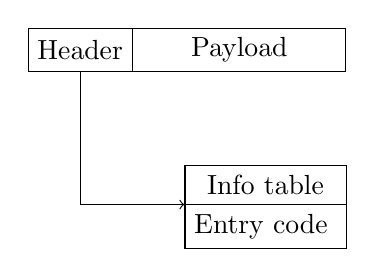
\begin{tikzpicture}[
		memory slab/.style={
			rectangle, draw,
		},
	]
		\node[
			memory slab, rectangle split, rectangle split parts = 2,
			rectangle split horizontal, align = center
		] (obj) at (0, 0) {
			Header
			\nodepart[text width = 70pt]{second} Payload
		};
		\node[
			memory slab, rectangle split, rectangle split parts = 2,
			align = center
		] (header) at (1, -2) {
			Info table
			\nodepart{second} Entry code
		};
		% for some reason, just (a) |- (b) doesn't work, even though (a) -| (b) works fine...
		\draw[->] (obj.one south) -- (obj.one south |- header.one split west) -- (header.one split west);
	\end{tikzpicture}
	\caption{The memory layout of a generic closure.}
	\label{fig:closure-layout}
\end{figure}

\textit{Closures} -- the runtime objects of programs compiled with
\acrshort{ghc} -- all share the same basic representation shown in figure
\ref{fig:closure-layout}. The \textit{header} contains primarily a pointer to
the metadata of a closure, though it also includes a profiling header if
profiling is enabled. The \textit{payload} of a closure usually contains data
not known at compile time. The \textit{info table} identifies the type of the
closure (data constructor, function, thunk, \ldots) and informs the garbage
collector about the pointer\-hood of the payload. The \textit{entry code} is
the code executed when \textit{entering}, i.e. evaluating the closure. For
example, the entry code of functions represents the body of the function.

The \acrshort{stg} uses a number of registers, a heap, and a stack which stores
function arguments and continuations. Closures can also reside statically in
the compiled object code of a Haskell program. During execution, any heap
allocations are preceded by a \textit{heap check}, which invokes garbage
collection if not enough space is left on the heap. Similarly, when code needs
to push values onto the stack, it performs a \textit{stack check} and grows the
stack if necessary.

All the dynamic allocations are managed by the garbage collector, including
stack frames and lightweight threads.

Here \todo{ew, improve the wording here} are a few of the most important
closure types:

\begin{description}
	\item[Function closures] represent Haskell functions. When entered,
		functions assume that all their arguments are present at the top of the
		stack. This is known as the \textit{eval/apply} evaluation model.

		The payload of function closures carries (pointers to) the free
		variables of the function's body.

	\item[Thunks] represent unevaluated expressions. When entered, the
		corresponding expression is evaluated and the closure is replaced with
		an indirection to the resulting value. This ensures that thunks are not
		evaluated multiple times, as subsequent attempts at evaluation will
		instead enter the indirection which will simply return the existing
		value.

	\item[Indirections] are proxies to other closures. Their payload is simply
		a single pointer to the target object. To reduce the overhead of
		sharing, indirections are removed by the garbage collector and never
		outlive the youngest generation.

	\item[Black holes] are indirections under evaluation. \todo{concurrent
		update}

	\item[Data constructors] carry their arguments (fields) as payload, ordered
		such that pointers come first. Their entry code returns immediately to
		the topmost stack frame (a constructor itself is always evaluated,
		although its arguments may not be).

	\item[Thread state objects] represent lightweight Haskell threads,
		including their stacks. Since a \acrshort{tso} is simply a closure, it
		is managed by the garbage collector, just like any other heap object.
		The garbage collector sends exceptions to blocked threads which become
		unreachable.
\end{description}


\subsection{Strictness features}
The compilation pipeline, the \acrshort{rts}, and base libraries are the
products of substantial amounts of effort invested over more than thirty years,
but they are not the only contributions of the \acrshort{ghc} project.
\acrshort{ghc} often serves as the incubator of new language features --
including those directly related to managing the amount of laziness in a
program. We dedicate this subsection to an overview thereof.

A simple and robust method of preventing undesired laziness is the
language extension \texttt{BangPatterns}, which introduces a new pattern syntax
\hsCode{!pat} for forcing an expression to \acrshort{whnf} before
pattern-matching it against \hsIdent{pat} \todo{we may need a
\texttt{\textbackslash hsPat}}. For short functions and clear algorithms which
do not benefit from pervasive laziness it is often very easy to simply annotate
certain patterns in the program with exclamation marks and observe a reduction
in memory consumption.

The language extension shares the exclamation mark syntax with a feature of
Haskell 2010, strictness flags\cite{haskell2010-strictness-flags}. While
\texttt{BangPatterns} add optional strictness to pattern matching, strictness
flags do the same \todo{find a better word} for data types. Unfortunately,
proper use of this flexibility hinges on the programmer's knowledge of how is
the particular piece of code going to be used. While it is good practice to
request the early evaluation of values which will have to be forced anyway,
sprinkling strictness annotations throughout library code in attempts to
prevent space leaks may lead to the unintentional sacrifice of the benefits of
laziness, even preventing some usage patterns in subtle ways. Additionally,
since these strict evaluation facilities only force thunks to \acrshort{whnf},
the evaluated objects may still retain large delayed expressions. The ability
to excise thunks from a Haskell value completely was the core motivation for
the development of the \hackage{deepseq} library.

The lack of programmer insight into how a piece of code is used in a program
and what strictness properties it has is a major developer experience issue.
Some of the discussed debugging tools help ameliorate the problem, but
\acrshort{ghc} itself includes features especially suited to doing so
\todo{wording?}. The compiler supports two profiling modes, cost-centre
profiling and ``ticky-ticky'' profiling, which the \acrshort{ghc} User's Guide
dedicates a chapter to\cite{ghc-profiling}. While the ``ticky-ticky'' mode is
only of interest to \acrshort{ghc} developers, the cost-centre profiling
functionality is an easy-to-use tool for understanding the time and space
behaviour of Haskell programs. All it requires of the programmer is a
recompilation of the modules of interest with a few specific compiler options.

Cost-centre profiling assigns the so-called ``cost-centres'' to certain
sections of code. The \acrshort{rts} records any time spent and allocations
performed during the evaluation of code associated with a cost-centre. These
recordings are summarised by a time and allocation profiling report, which the
profiled program generates. The report indicates the time and space
requirements of each cost centre in proportion to the entire program.
\acrshort{ghc} is able to introduce cost centres automatically by adding them
to all non-in\-lined bindings, but the user also has the option to annotate
terms with a pragma to fine-tune the placement of cost centres.

\acrshort{ghc}'s implementation of profiling can shed some light on the use of
call-by-need in a Haskell program. The compiler can also provide certain deeper
insights about the program's strictness, although it presents them in a
substantially less user-friendly manner. In particular, \acrshort{ghc} can
output the translation of surface syntax to its internal language, Core. Being
a fairly small $\lambda$ calculus, Core has a clearer semantics including a
strict pattern-matching operator \hsCode{case e of arms...}, which indicates
obviously strict subexpressions. Furthermore, the Core output features
\textit{demand signatures}, inferred by \acrshort{ghc}'s demand
analysis\cite{cmtary-demand-analysis}, which classify binders depending on how
strict they are in their arguments and to what extent do they use the
components of arguments of product types. The results of demand analysis are
crucial for subsequent optimisation. Understanding the demand signatures of a
program can equip the programmer with the information necessary to determine
which patterns would most benefit from the \texttt{BangPatterns} extension,
which data types could be annotated with strictness flags, and which parts of
the program should be refactored in other ways in order to improve the native
code generated by the compiler.

The \acrshort{ghc}-provided tooling outlined above -- particularly the option
to dump Core code during compilation and analyse demand signatures -- is rather
obscure. It is reasonable to expect the average Haskell programmer to only
reach for the profiling tools in a time of dire need, when writing
high-performance code or dealing with unacceptable space leaks. It is further
reasonable not to expect the average Haskell programmer to know the internals
of the compiler well enough to ask it for the Core representation of their
program, or indeed to be aware at all of the existence of demand signatures,
which are only described in the \acrshort{ghc} Commentary\footnote{
	The commentary is intended for \acrshort{ghc} developers and is hosted on a
	GitLab instance (online), unlike the User's Guide which is bundled with the
	\acrshort{ghc} distribution and revised for every release.
}. Perhaps it would be interesting to include the strictness information
inferred by the compiler in interfaces programmers often interact with, such as
the various widgets provided by the \acrfull{hls} \cite{gh-hls}, but
to our knowledge no such tool exists at the time of writing.

In theory, the \acrlong{ghc}'s optimisations are advanced enough to compile the
majority of Haskell code fairly efficiently, without space leaks or allocation
slow-downs, while enabling the greater flexibility, code reuse, and abstraction
of a non-strict language. However, inefficiencies introduced to support
unnecessary laziness which are small enough not to cause substantial problems
could hide in the compiled program. It is a part of the motivation behind this
thesis to lay the groundwork necessary for their detection.

\todo{Explain that several previous approaches had a direct influence on the
	compiler. \acrshort{ghc} now has \acrshort{hpc}-specific features, compiler
	plugins, which supersede source-to-source transformations (strengthening
	the monopoly but simplifying implementation and streamlining the process),
	and a codebase that's increasingly amenable to various extensions via the
	trees that grow pattern, \hsIdent{Tickish}, etc.}
...


\chapter{Analysis and design} \label{sec:analysis-design}

\section{Overview} \label{sec:analysis-overview}
\begin{itemize}
	\item add a proper problem statement
	\item summarise possible approaches
	\item detail \acrshort{ghci}
	\item detail compiler plugins
	\item build on \texttt{Tickish}
\end{itemize}

\section{Approach} \label{sec:approach}

The goal of this work is to design and implement a tool suitable for
understanding how is laziness used in real-life Haskell programs. To analyse
the practical implications of \acrshort{ghc}'s implementation of non-strict
semantics, we have to understand the strictness properties of functions. For
example, some arguments may be evaluated if and only if others are. The tool
must capture these dependencies and usage patterns, as they may uncover both
use cases where laziness is essential and places where it could be safely
avoided, even though static analysis cannot determine so.

Dynamically inferring the strictness properties of functions requires a peek
under the hood of Haskell's runtime machinery. Typical Haskell code is
oblivious to the underlying representation of the values it manipulates, as
reification of the heap objects underneath the abstractions would weaken
equational reasoning and parametricity.

Once we have the power to inspect the runtime representations of values, we
need to use it to determine the strictness of functions. A function \hsIdent{f}
is strict in an argument \hsIdent{a} if \hsIdent{a} has to be evaluated
whenever \hsCode{f a} is evaluated.

There is a number of possible approaches to this problem. As discussed in
chapter \ref{sec:state-of-the-art}, there already exist related projects which
we could build on, at various levels of abstraction. At the lowest level, we
could modify the \acrshort{rts} and extract information about heap objects
there. We could also modify the compiler in various ways, since it already
includes support for \acrshort{hpc} and profiling, which is similar to the
tracing we would like to implement. Another option is to follow the path of
\nameref{sec:hat}, rewriting the textual source code of traced programs. In
this work, we explore two design directions: extending \acrshort{ghci} and
tracing with compiler plugins.

\section{Using \acrshort{ghci}} \label{sec:using-ghci}
The bytecode compilation pipeline and the interpreter offer a refreshing break
from the comparative complexity of \acrshort{ghc}'s back end. Unlike the
\acrshort{rts} linked to a program compiled to object code, the interpreter is
at the perfect level of abstraction to directly track evaluations of thunks and
the stream of control flow in a program.

One of the issues with this approach that is clear from the outset is the range
of supported language extensions. The bytecode compiler and the interpreter
lack support for un\-box\-ed tuples and sums, shrinking the set of programs the
tracer would be able to analyse. In our design of a \acrshort{ghci}-based
solution, we took inspiration from \cite{emp-study-laziness-r}, which modified
the virtual machine of the R language.

Before we describe the \acrshort{ghci} tracing modifications, let us take a
closer look at how this part of the compiler project works. \acrshort{ghci} is
an interactive interface built on \acrshort{ghc}'s bytecode compilation
pipeline and the bytecode interpreter of the \acrshort{rts}. It offers a
read-eval-print loop popular in other functional programming languages.

\acrshort{ghci} consists of several key components: the \acrshort{ghci} UI, the
\acrshort{ghci} library code, the \acrshort{ghci} debugger, the bytecode
generator, and the bytecode interpreter.  The following sections will introduce
each of the building blocks from which \acrshort{ghci} is composed, starting
with an overview of how they fit together.

\subsection*{The life of an interpreted expression}
\acrshort{ghci} can either serve as a \acrshort{repl} interface, processing
expressions one by one, or as an alternative compilation and execution
environment for entire modules. These two modes can be freely mixed. The
backbone of \acrshort{ghci} is a modified \acrshort{ghc} pipeline which
culminates in bytecode generation, producing a collection of bytecode objects
together with high-level information about breakpoints, pointers to allocated
string literals, and other data.

Compiled\footnote{That is, compiled to bytecode instructions.} bytecode objects
and their metadata form an analogy of the compiler's module abstraction called
\hsType{CompiledByteCode}. \acrshort{ghci} includes a dynamic linker capable of
resolving references between bytecode objects as well as between
\acrshortpl{bco} and object code.

These features are transparent to the user, who manipulates \acrshort{ghci} via
its user interface. The UI is implemented separately from the core
functionality and communicates with the \acrshort{ghci} library code via
message-passing. This separation allows the UI and the library code, which is
in charge of interpreted evaluation, run in different processes.
\acrshort{ghci} features a mode of operation called ``Remote \acrshort{ghci},''
in which the UI and the interpreter communicate over a pipe. Remote
\acrshort{ghci} is useful for situations where the capabilities and heap object
definitions of the runtime systems of the compiler and the interpreter differ,
e.g. when the compiler and \acrshort{ghci} UI were built regularly with
optimisations, but the interpreter was built with profiling.

When evaluating an expression, the library code forks a new thread to perform
evaluation independently of the interpreter server. This ensures that
exceptions raised during evaluation of an expression do not crash
\acrshort{ghci}. The server forwards exception handlers appropriately to ensure
this is the case. The two threads communicate via \textit{mutable variables},
or \hsType{MVar}s. These are concurrency primitives from the
\hsModule{Control.Concurrent.MVar} module which effectively implement
concurrent, mutable \hsType{Maybe}s\cite{concurrent-haskell}. A mutable
variable of type \hsType{MVar a} contains either no values or a single value of
type \hsType{a}. It can be safely shared across threads and supports
operations \hsIdent{takeMVar} and \hsIdent{putMVar}. The former operation
extracts the value stored in an \hsType{MVar}, leaving the variable empty if a
value is present. If the variable is empty, the operation blocks. The
complementary operation \hsIdent{putMVar} blocks on a full variable and fills
it with a value as soon as it is empty.

Two \hsType{MVar}s play an important role in the design of \acrshort{ghci},
\hsIdent{statusMVar} and \hsIdent{breakMVar}. These variables form a
communication channel between the server thread and the thread responsible for
the evaluation of an expression, which we will call the \texttt{eval} thread.

When the server thread forks into the \texttt{eval} thread to begin expression
evaluation, it waits on the \hsIdent{statusMVar}. The \texttt{eval} thread
keeps running, eventually either producing a result, throwing an exception, or
hitting a breakpoint. In the former two cases, it simply fills the
\hsIdent{statusMVar} with the appropriate information (either the result of
evaluation or the exception) and exits. The server thread resumes execution,
passing the result from the \texttt{eval} thread to the UI.

The case when the \texttt{eval} thread hits a breakpoint is more interesting.
First, the \texttt{eval} thread fills the \hsIdent{statusMVar} to wake the
server thread, notifying it of the breakpoint. Then it waits until the server
thread fills the \hsIdent{breakMVar}, pausing evaluation. The server thread
notifies the UI, passing along an identifier of the breakpoint that the
\texttt{eval} thread hit. At this point, the UI notifies the user that
evaluation paused on a breakpoint. The user can continue to enter expressions
into the \acrshort{ghci} prompt, these will be evaluated independently by newly
forked threads. These can also hit breakpoints and wake the server thread,
which notifies the UI again. None of this interferes with the initial
\texttt{eval} thread, because every forked \texttt{eval} thread gets a new pair
of status and breakpoint mutable variables. The user may resume execution in
the UI, which messages the server thread, which in turn fills the appropriate
\hsIdent{breakMVar}, waking the \texttt{eval} thread and blocking on
\hsIdent{statusMVar} once again.

\subsection*{Bytecode generation}
The bytecode facilities of \acrshort{ghc} involve a detour from the typical
sequence of steps performed to transform Haskell sources all the way to a form
suitable for linking or execution. After desugaring, the program is transformed
directly into bytecode instructions\footnote{Note that this approach will soon
be replaced by a new bytecode pipeline which follows the usual compilation
process all the way to \acrshort{stg}\citationNeeded.}. Optimisations
implemented in the simplifier are not performed. \acrshort{ghci} is intended
for interactive evaluation and favours fast, iterative development over runtime
performance, making the naive code generation approach a reasonable choice.

Every top-level definition, every scrutinee of a \hsCode{case} expression, and
every right-hand side of a non-trivial \hsCode{let} expression are compiled to
a \acrfull{bco}. Such an object contains an array of bytecode instructions
together with the data typically associated with a heap object: the arity of
the \acrshort{bco}, a bitmap indicating which of its arguments are pointers,
the literals it refers to, and pointers to various objects it refers to
(symbols, primitive operations, other \acrshortpl{bco}, or the object's array
of breakpoint information).

The bytecode format comprises 67 instructions in total, 35 of which only exist
to provide various ways of pushing values to the stack. The rest of the virtual
instruction set consists of a few instructions for heap allocation, various
less-than and equality tests, two instructions for invoking the C
\acrshort{ffi}, an explicit stack check instruction, and others. The wide
variety of instructions of a shared or similar purpose, particularly in the
case of stack pushes, is the consequence of distinguishing between the
representation of their arguments -- arguments can be pointers subject to
garbage collection, word-sized integers, 64bit integers, floating point and
double precision numbers, etc.

There is one particular instruction that catches the eye: \texttt{BRK\_FUN}.
The bytecode generator places \texttt{BRK\_FUN} instructions at the very
beginning of every bytecode object. These instructions correspond to
breakpoints, though they are only relevant when the user has ``placed'' a
breakpoint at a position in the source code. Alas, ``placing'' breakpoints is
something of an illusion, the instructions are pervasive and every breakpoint
has a numeric identifier assigned at compilation time. The introduction of a
new breakpoint in the \acrshort{ghci} UI simply sets a flag in a breakpoint
bitmap, enabling the corresponding breakpoint instruction from the perspective
of the interpreter.


\subsection*{The bytecode interpreter}
The interpreter which \acrshort{ghci} relies on is a part of the
\acrshort{rts}. Its primary workhorse is the \texttt{interpretBCO} function
which handles closure evaluation, unboxed returns, function application, and
interpretation of bytecode instructions. For tasks it is unable to deal with,
such as application of machine-code functions, it returns to the scheduler.

Interpretation works simply by case analysis on the current instruction.

\subsection*{The debugger}
\todo{this needs an update now that the previous subsections were rewritten}
\todo{don't forget to mention the feature where you can print the runtime
values of things while paused at a breakpoint}

A notable feature of \acrshort{ghci} is its debugger, which allows the
programmer to place breakpoints on certain expressions in their code. The
interpreter then pauses execution when it is about to evaluate an expression
marked by a breakpoint.

Due to laziness, the order in which breakpoints are hit depends on the order in
which their respective thunks are forced to \acrshort{whnf}, not directly on
the order in which functions are called. Breakpoints thus equip the Haskell
programmer with a powerful tool for debugging order of evaluation issues caused
by the language's non-strict semantics.

Internally, breakpoints rely on a special bytecode instruction called
\texttt{BRK\_FUN}. Upon encountering this instruction, the interpreter first
checks whether it is already returning from a breakpoint (via a flag in the
\acrshort{tso}). If it is not returning from a breakpoint and the associated
breakpoint is enabled, the interpreter pauses execution at this point.

Pausing on a breakpoint is quite an involved action. The interpreter prepares
to call an ``IO action,'' which is a Haskell function invoked to resume
\acrshort{ghci}'s UI thread by filling the shared mutable variable. This
preparation saves the top stack frame to a new closure, a pointer to which is
passed to the IO action. The stack is then set up to call the IO action, and
the interpreter returns to the scheduler in order to perform the call.

At no point is the instruction pointer persisted -- the progress of evaluation
of the current \acrshort{bco} is lost whenever the interpreter stops at a
breakpoint. This is acceptable, as the bytecode generator makes sure to only
put \texttt{BRK\_FUN} instructions at the very start of bytecode objects and
the \acrshort{tso} flag ensures that a just-visited breakpoint is not stopped
at again.

\subsection*{Trace\-points}
Our design for dynamic tracing via \acrshort{ghci} builds on the existing
functionality of breakpoints. We introduce \textit{trace\-points}, a simpler
variant of breakpoints which uses the communication channel between the server
and \texttt{eval} threads to pause evaluation at every breakable expression.

\subsection*{Summary}
\todo{\ldots}


\section{The compiler plugin approach}
To produce useful tracing output, a dynamic tracing framework must capture
interesting events during a program's evaluation and relate them to one
another. In particular, the evaluation of function arguments must be clearly
related to the respective function call to enable reasoning about the
strictness of a function on a call-by-call basis. While retaining the order of
evaluation is trivial in a call-by-value language, laziness introduces
interleaving. This can only be dealt with by the introduction of state into the
program (or into the tracing framework) in order to recover the dependencies
between function calls and argument evaluations, which are no longer implicit
in the order of the trace events.

It is this function-call-specific state that becomes difficult to express
without high-level information about the program structure at hand, as was the
case with the \acrshort{ghci} approach described in section
\ref{sec:using-ghci} \todo{maybe ``the previous section?'' Susceptible to
problems when reordering though}.

\subsection*{Adding state}
\todo{A manual introduction of state into the program is rather trivial\ldots}

Fortunately, function-call-specific state can be easily introduced into the
source program, simply as local variables. It suffices to keep a unique
identifier of the particular function call that the argument evaluation traces
can refer to. Such a unique identifier necessarily needs to change with every
function call. In clean Haskell code without unsafe features, this is
impossible in general, as the language requires the use of the \hsType{IO}
monad in order to perform side-effecting computations.

Since rewriting functions into a monadic form would be a difficult undertaking,
we prefer the way of unsafe features. Integer counters are enough for call
identification purposes, so we choose to keep one counter per function. All
counters can be stored in a single mutable map, which associates

\todo{
to-dos:
\begin{itemize}
	\item describe the general idea of the source plugin
	\item explain the use of SYB
	\item explain the use of TH and splicing
	\item explain how the global mutable map resides in the plugin's module
	\item explain the difficulty of trying to implement similar functionality
		in a core plugin instead
\end{itemize}
}

Equipped with a means of introducing benign side-effects into programs for
tracing purposes, we are in search of a way of rewriting source code to put
these side-effects to use. One plausible approach would be direct source code
rewriting, akin to \nameref{sec:hat}. As described in section
\ref{sec:existing-tools}, source-to-source transformations have the benefit of
generality, but also the downside of additional complexity in both the
rewriting process itself and the build process of the program, which the user
of our tool would have to deal with. Furthermore, true implementation
agnosticism of the tracing framework would require compiler-independent support
for inspection of the Haskell heap, for which no solution seems to exist at the
time of writing\todo{right?}. A less general but more ergonomic way of
rewriting source code is via \acrshort{ghc}'s \textit{source plugins}, which
hook directly into the compiler pipeline and can operate on the surface-level
syntax at different stages.

\subsubsection*{Source plugins}
Source plugins\cite{ghc-source-plugins} are a relatively recently introduced
feature of \acrshort{ghc}. Compiler source plugins are Haskell packages which
invoke the \acrshort{ghc} API\todo{same as UI, I suppose?} to hook into the
compiler pipeline and modify the compiled program at various stages of the
front-end. Unlike Core plugins\citationNeeded, which operate on the internal
language, source plugins deal with the entirety of Haskell's surface syntax.

Rather than parsing, transforming, and serialising the source code separately
to the compilation step, we can design a plugin that performs the required
source transformations in the compiler pipeline directly. We introduce two
tracing functions, \hsIdent{traceEntry} and \hsIdent{traceArg}, into the
current module. We then rewrite the source program to call \hsIdent{traceEntry}
every time a function in the program is invoked and we thread every reference
to a function's argument through \hsIdent{traceArg}. This introduces the
opportunity to inspect the runtime representations of the arguments passed to a
function when the result of the function is under scrutiny.

We can determine the strictness properties of a transformed function from the
calls it makes to the tracing utilities. If we record a call to a (transformed)
top-level function \hsCode{f :: Int -> Int -> Int} defined as \hsCode{f x y =
...} via \hsIdent{traceEntry} but no calls to \hsIdent{traceArg}, the
function makes no use of any of its arguments, and is therefore non-strict in
both of them. Examples of functions of this behaviour include \hsCode{f x y =
3}, \hsCode{f x y = undefined}, or \hsCode{f x y = f x y}. Note that the latter
example references the arguments on the \acrshort{rhs}, but these references are
never evaluated. If a call to \hsIdent{f} is followed by a call to
\hsIdent{traceArg} for the \hsIdent{x} argument, but the program terminates and
no calls to \hsIdent{traceArg} for the \hsIdent{y} argument occur, we say that
\hsIdent{f} is strict in \hsIdent{x} and \textit{potentially non-strict} in
\hsIdent{y}. \hsIdent{f} could be non-strict in \hsIdent{y}, but it could also
conditionally require \hsIdent{y} to be evaluated based on the value of
\hsIdent{x}. The property of a multi-argument function being strict in one
argument if another argument matches a predicate (and being non-strict in that
argument otherwise) is what makes the interpretation of traces of nested
functions tricky.

\subsection*{Rewriting the \acrshort{ast}}
Armed with the necessary tracing functions and a plan on how to apply them, we
move on to the problem of syntax tree transformation. The \hsModule{GhcPlugins}
module\cite{hkg-ghcplugins} of the \acrshort{ghc} \acrshort{api} includes the
necessary functions to hook into the compiler pipeline. A source plugin can
choose to modify the syntax tree at three different stages: right after
parsing, between renaming and typechecking, or just after the typechecker has
run. These hooks involve different trade-offs. Construction of new (sub)trees
becomes more and more difficult further down the pipeline as the internal
representation accumulates metadata from the various stages. On the other hand,
the available metadata may be necessary for certain tasks and can help plugin
authors write more robust implementations. For example, constructing parsed
expressions is almost as easy as writing the surface syntax in a source file,
using strings as identifiers, but it may result in accidental captures of
bindings in scope. Because the renaming phase disambiguates identifiers,
constructing renamed \acrshortpl{ast} avoids this issue, at the expense of
either working with abstract identifiers, or invoking a renaming phase
manually.

\todo{fix \texttt{\textbackslash citeauthor}}
As \citeauthor{blog-source-plugins}'s introduction to source plugins shows, the
costs associated with the construction of syntax trees later in the pipeline
are not prohibitive\cite{blog-source-plugins}. The \acrshort{ghc}
\acrshort{api} exports high-level functions which let the plugin author take
trees from parsed to renamed to typechecked in only a few lines of code.
Moreover, the plugin author can use the quasi\-quoting
features\cite{th-quasiquoting} of Template Haskell\cite{th-classic} to greatly
simplify the construction of expressions. The quasi\-quoting facilities even
manage references to definitions in the scope of the plugin's source code
automatically. Common patterns in the expressions created by the plugin can be
included as regular top-level definitions in the plugin's module or in a module
the plugin depends on and spliced into the syntax tree. With these high-level
features in mind, the suitable injection mechanisms for a dynamic tracing
source plugin seem to be before and after typechecking. We only discuss the
latter approach in the following text, even though a source plugin operating on
the renamed \acrshort{ast} would likely be very similar. Note that the
\acrshort{api} makes no hard distinction between the different approaches to
pipeline extensions. Indeed, a source plugin simply provides a value of the
\hsType{Plugin} data type, overriding the appropriate fields of a default
plugin implementation with monadic functions. A source plugin could run custom
code after each of the frontend stages.

The actual process of rewriting the right-hand sides of function definitions
involves the data types for the surface syntax of Haskell, which has hundreds
of constructs\cite[Key~Design~Choices]{arch-ghc}. The general task of
transforming hierarchies of deeply nested data types has many innovative
Haskell solutions, including optics and generic programming. While we could use
pro\-functor optics or novel generic approaches, we leverage a fairly simple,
if a bit dated, generic programming technique via the \acrfull{syb}
library\cite{syb-paper}. \acrshort{syb}'s built-in querying and transformation
schemes empower the Haskell programmer with means of applying type-specific
functions in all appropriately typed fields of a nested data structure. The
library is built using powerful generalisations of folding and a number of
combinators, making it easy to create new traversal schemes as compositions of
existing building blocks.


\chapter{Implementation}
In this chapter, we confront some of the development-related issues that tend
to arise when working with the \acrshort{ghc} project, in the hope of easing
future endeavours. The description of the problems we encountered in our work
relates to features of the compiler which did not fit in earlier chapters.
Next, we discuss the implementation details of a compiler source plugin we
developed for dynamic tracing and present the results of the implementation.


\section{Working with \acrshort{ghc}}
While obtaining and compiling a local copy of \acrshort{ghc} source code is
unnecessary for compiler plugin development, a programmer inexperienced with
the internals of the project may find it helpful to occasionally peek under the
hood of its \acrshortpl{api}. Obtaining a working copy is also a prerequisite
for forking\todo{term?} the project -- we did so when evaluating the
\acrshort{ghci} approach.

The \acrshort{ghc} codebase is a large and complicated collection of source
files written primarily in Haskell and C\cite{arch-ghc}. The ever-evolving
project is supported by a custom build system called Hadrian\cite{hadrian},
itself written in Haskell, introduced to replace \acrshort{gnu} Make.
Additionally, the build tool of the programmer's choice can be combined with a
Docker or Nix -assisted set-up, simplifying the installation of other
dependencies required for the build process. We do not recommend using Make:
Hadrian was developed to address many issues with Make, including its excessive
complexity and poor performance.  Tools for simplifying library management
(particularly Nix and Docker) are compelling choices for projects with larger
teams. However, we found it significantly easier to set up a ``native''
development environment. Both Nix and Docker suffer from substantial disk usage
overheads. Our experience in developing a Docker container for \acrshort{ghc}
8.10.2 indicates that large portions of the native set-up have to be replicated
in the container.

For example, correctly configuring \acrshort{hls} to load the \acrshort{ghc}
source code is quite an involved task, eased by the \texttt{hie-bios}
project\cite{gh-hie-bios} which ships with Hadrian (as a part of the
\acrshort{ghc} source tree). However, compiling \acrshort{ghc} inside the
container results in \texttt{hie-bios} reporting include paths specific to the
container's file\-system to the language server, which in turn breaks all of
its functionality. One possible solution is installing the \acrshort{hls}
inside the Docker container instead and letting the code editor of choice talk
to the containerised process. In comparison, a native set-up with
\texttt{ghcup} is far easier and comes with fewer surprises along the way,
which is why we would recommend it for a project similar in scale to ours.

\subsection*{Build process}
The build system bootstraps the self-hosting compiler in
several steps. To build \acrshort{ghc}, an appropriate version of
it has to be already installed. The compiler provided by the system is referred
to as the \textbf{stage 0} compiler \todo{fix the formatting of stages}.
\acrshort{ghc} comes with build scripts which use the \textbf{stage 0} compiler
to build first the Hadrian build system. Once Hadrian has been built, the user
invokes it to build the \textbf{stage 1} compiler, which is a \acrshort{ghc}
linked against the \textbf{stage 0} \hackage{base} library. The \textbf{stage
1} compiler is subsequently used to build the core libraries from scratch. It
is then utilised again to build the \textbf{stage 2} compiler, which is linked
against the freshly built \hackage{base}. The \textbf{stage 2} compiler
constitutes a complete build of \acrshort{ghc} from source code. There is an
optional follow-up step, where the \textbf{stage 2} compiler builds a
\textbf{stage 3} compiler, which is useful for profiling \acrshort{ghc} while
building \acrshort{ghc}.

The first step to working on the project after obtaining the source code is
setting up the build system. Since specific releases of \acrshort{ghc} require
specific \textbf{stage 0} compilers as the project quickly adapts to use new
language extensions, the management of \acrshort{ghc} versions on a Unix-like
system with a system-wide package manager can be difficult. To ease the
management of installed versions and enable quick switching between them, the
\texttt{ghcup} tool\cite{ghcup} has been developed. \todo{this will need some
more citations} \texttt{ghcup} lets the \acrshort{ghc} developer quickly
install and switch between the releases of not only \acrshort{ghc} itself, but
also Cabal, the Haskell build system and dependency manager, and the
\acrfull{hls}, an \acrshort{lsp}-compliant language server providing
Haskell-specific editor integration features.


\todo{ways and flavours!}
After the initial build, the \textbf{stage 1} compiler can be \textit{frozen}
by passing a flag to the build system on subsequent invocations. This prevents
rebuilding the \textbf{stage 1} compiler every time a source file changes, which
speeds up the edit-compile-run cycle tremendously.

\todo{\ldots}

\section{Dynamic tracing with plugins}
\todo{\ldots}

\subsection*{Anatomy of a plugin}
Our source plugin consists of four modules.
\begin{itemize}
	\item \hsModule{TracingPlugin}, the entry point of execution and the only
		exposed module of the package,
	\item \hsModule{Typechecking}, which contains utilities for typechecking
		expressions constructed by the plugin,
	\item \hsModule{Logging}, which defines the tracing functions that we
		compile into source programs, and
	\item \hsModule{Rewriting}, where the magic happens. \todo{perhaps
		unprofessional}
\end{itemize}

The \hsModule{TracingPlugin} module simply defines and exports a
\hsType{Plugin} derived from the \hsIdent{defaultPlugin} implementation,
overriding \hsIdent{typeCheckResultAction}, the function invoked after the
typechecking phase. Neglecting command-line arguments, our action has the type
\hsType{ModSummary -> TcGblEnv -> TcM TcGblEnv}. As the type indicates, it
computes within the typechecking monad (\hsType{TcM}) with access to
information about the current module (\hsType{ModSummary}), modifying its
typechecking environment (\hsType{TcGblEnv}). The action is invoked once for
each compiled module. The typechecking environment is a large data structure
which describes the top level of a module with 58 fields. Of these, only
\hsCode{tcg_binds :: LHsBinds GhcTc} is interesting to us. The type
constructor \hsType{LHsBinds} stands roughly for ``located Haskell bindings''
and represents a collection of all the top-level bindings of a module annotated
with their source file locations. Our post-typechecking action simply threads
this field through our rewriting function, which also computes in the
typechecking monad, and returns the transformed bindings.

The rewriting function, shown in figure \ref{fig:hs-rewrite}, resides in the
\hsModule{Rewriting} module. It initiates a stateful computation which
transforms the bindings in a generic manner using the \acrshort{syb} library.
\begin{figure}[h]
	\centering
	\begin{minted}[autogobble]{haskell}
        rewrite :: LHsBinds GhcTc -> TcM (LHsBinds GhcTc)
        rewrite binds = fst <$> (`runStateT` initialState)
                                (everywhereM' trans binds)
	\end{minted}
	\caption{The top-level rewriting function, a sole export of the
	\hsModule{Rewriting} module.}
	\label{fig:hs-rewrite}
\end{figure}

Since the \acrshort{ghc} \acrshort{api} abstracts over compiler state using
(among other types) the \hsType{TcM} monad, the generic transformation
involving any non-trivial compiler computations needs to be monadic as well.
This transformation is implemented by the \hsIdent{trans} function (shown in
fig. \ref{fig:hs-trans}), which additionally carries a context from the roots
of the top-level definitions down to their leaves. We combine the stateful
traversal with the typechecking monad by way of the \hackage{mtl} package,
itself inspired by \cite{higher-order-polymorphism}, using the \hsType{StateT}
monad transformer.

\begin{figure}[h]
	\centering
	\begin{minted}[autogobble]{haskell}
        trans :: Typeable a => a -> StateT WrapperState TcM a
        trans = mkM collectFunInfo `extM` wrapRef `extM` incrementCC
	\end{minted}
	\caption{The generic transformation function.}
	\label{fig:hs-trans}
\end{figure}

\hsIdent{trans} is applied in a single, top-down traversal of the
\acrshortpl{ast} via a \acrshort{syb} scheme derived from \hsIdent{everywhereM}.
Ultimately, the function pattern-matches on important structures in the syntax
trees of top-level bindings in three different ways:
\begin{enumerate}
	\item \hsIdent{collectFunInfo} adds information about the current function
		to the \hsType{WrapperState},
	\item \hsIdent{wrapRef} wraps argument references with a tracing function, and
	\item \hsIdent{incrementCC} wraps the right-hand side of each function with
		a \hsCode{let} binding, introducing a call counter variable into
		its scope.
\end{enumerate}

Each of these building blocks of the complete transformation operates slightly
differently.

\begin{description}
	\item[\hsCode{collectFunInfo :: Bind -> StateT WrapperState TcM Bind}]
		pattern-matches on the various sorts of bindings that can appear in an
		\acrshort{ast} and extracts the names of the named ones, saving them to
		the \hsType{WrapperState} context, thus providing the name of the
		innermost named function to the other transformations.

	\item[\hsCode{incrementCC :: RHS -> StateT WrapperState TcM RHS}]
		pattern-matches on right-hand sides of functions and introduces calls
		to the tracing function \hsIdent{traceEntry} using \acrfull{th}.
		Calling \hsIdent{traceEntry} with a function name increments a global
		call counter for that function and returns the counter's current value.
		\hsIdent{incrementCC} has to introduce a new binding in the scope of
		the right-hand side so that tracing calls on the \acrshort{rhs} can
		refer to the call ID.  Since \acrshort{th} cannot lift the Haskell
		\acrshort{ast} types, the binding has to be constructed in two steps.

		First we read the \hsType{WrapperState} to find out the name of the
		function we are currently transforming. We construct a \acrshort{th}
		expression for the application of \hsIdent{traceEntry} to the function
		name and bind it via a \hsCode{let} binding which assigns the result to
		a new call counter variable in the scope of a dummy expression (a proxy
		to \hsIdent{undefined}). Then we typecheck this expression and run a
		\acrshort{syb} transformation which replaces the dummy subexpression
		with the original right-hand side. Care must be taken when replacing a
		node in the typechecked \acrshort{ast} because the typechecker inserts
		type applications for polymorphic terms such as \hsIdent{undefined}.

		Finally, \hsIdent{incrementCC} also finds the \hsType{Id} of the call
		counter variable via a \acrshort{syb} query and saves it in the
		\hsType{WrapperState}.

	\item[\hsCode{wrapRef :: LExpr -> StateT WrapperState TcM LExpr}]
		pattern-matches on references to function arguments in function bodies.
		Its purpose is to transform every argument reference into a call to
		\hsIdent{traceArg}.

		\todo{fix \texttt{\textbackslash hsCode} overflows}

		To identify references to function arguments, \hsIdent{wrapRef}
		consults the \hsCode{boundVars :: [Id]} collection. This collection is built
		independently of the \hsIdent{wrapRef} transformation, since it needs
		no function-specific information. We rely on the fact that while
		references to bindings are semantically valid only in local
		(lexically-scoped) contexts, they have globally unique identifiers.
		Collecting the identifiers of function arguments is thus a simple task
		of traversing all the syntactical pattern-matching structures which
		bind them. We once again leverage \acrshort{syb} to do this without
		having to pattern-match on the entirety of surface syntax.

		When the reference wrapping transformation identifies a function
		argument, it constructs a partial application of the \hsIdent{traceArg}
		tracing function and applies the original binding reference to it. The
		partially-applied \hsIdent{traceArg} is an unsafe identity function
		which logs information about the argument's runtime representation to a
		file.

		Since the overall rewriting operation proceeds in a top-down manner,
		the \hsIdent{wrapRef} transformation runs into the issue of producing
		subexpressions it could recursively match on again. This could be
		avoided by tagging the transformed expressions somehow. Unfortunately,
		this is difficult to achieve, because the \acrshort{ast} datatypes lack
		useful typeclass instances for doing so. Crucially, there is no notion
		of equality on syntax trees and no hashing implementation which would
		let us store the transformed expressions in a hash set (or at least a
		set). We work around this limitation by stripping the source location
		tags from the \acrshort{ast} nodes and checking for their presence
		before invoking \hsIdent{wrapRef}'s rewriting logic, but we are aware
		of the problems with this approach. However, issues with error
		reporting are largely mitigated by the fact that the plugin is invoked
		after the source program passed the typechecking phase.
\end{description}

\subsection*{Implementation of tracing utilities} \label{sec:tracing-util-impl}
The tracing functions inserted into the \acrshort{ast} by the rewriting logic
reside in the \hsModule{Logging} module. They leverage the unsafe IO features
of Haskell, specifically the standard \hsCode{unsafePerformIO :: IO a -> a}
from \hsModule{System.IO.Unsafe}, to hide the side-effects of tracing from the
type system. When invoked, these functions append a row of
\acrshort{csv}-encoded data to a \textit{trace file}, a log of interesting
events that occurred during the evaluation of a Haskell program, which is
suitable for further analysis.

\begin{description}
	\item[\hsCode{traceEntry :: String -> Int}] marks the evaluation entry
		point of a function. Taking the function's name, it increments its call
		counter in the background and returns its new value. The call counters
		are stored in a global map called \hsCode{functionEntries :: IORef (Map
		String Int)}. The \hsType{IORef} indirection makes
		\hsIdent{functionEntries} a mutable variable which can be manipulated
		in the \hsType{IO} monad. The map is explicitly marked with a
		\mintinline[
			breakbytokenanywhere,breaklines
		]{haskell}|{-# NOINLINE #-}|
		pragma to ensure it is shared between the tracing calls. Since the
		\hsType{IORef} constructor returns a reference in the \hsType{IO}
		monad, we allocate the global variable via \hsIdent{unsafePerformIO}.

		The call counter map is empty at first, individual counters are
		initialised on-demand. The initialisation of a new call counter and the
		increment of an existing one are both described concisely by the
		\hsIdent{insertWith} operation on \hsType{Map}s, which takes a binary
		function on values, a key, an initial value, and a map, and either
		initialises the key to the initial value or updates it by applying the
		binary function to its current value and the initial one. This
		operation is applied atomically via \hsIdent{atomicModifyIORef'} to
		accommodate concurrent updates.

	\item[\hsCode{traceArg :: String -> String -> Int -> a -> a}] indicates a
		reference to a function argument. Partially applying this function to
		the name of the enclosing function, the name of the referenced
		argument, and the number of the call to the enclosing function leaves
		an impure identity, which is applied to the actual argument.
		\hsIdent{traceArg} leverages the \hackage{ghc-heap-view} library to
		take a peek at the runtime representation of the argument to determine
		whether it has been evaluated or not.

	\item[\hsCode{logt :: TraceSort -> [String] -> IO ()}] persists a tracing
		message to the trace file. Calls to this function are not introduced
		during the rewriting process directly, but both \hsIdent{traceEntry}
		and \hsIdent{traceArg} call it internally. The function can thus stay
		in the safe realm of the language, as its type indicates. File system
		operations in Haskell require a value of type \hsType{Handle} which the
		\acrshort{rts} uses to manage IO with file system objects. Allocating a
		handle corresponds to opening a file. Since that is a potentially
		expensive operation, we store the handle in another non-in\-line\-able
		\hsType{IORef}, again created globally with \hsIdent{unsafePerformIO}.
		\hsIdent{logt} then simply reads the \hsType{IORef}, appends tracing
		data to the file, and flushes the handle, to avoid problems with lazy
		IO and prevent data loss when the program exits.
\end{description}



\setsecnumdepth{part}
\chapter{Conclusion}
...

\bibliography{./bibliography/bbl.bib}
\bibliographystyle{./styles/iso690.bst}

\setsecnumdepth{all}
\appendix

\printglossary[type=\acronymtype]


\chapter{Contents of enclosed CD}

\todo{figure out what to do about this}
%change appropriately

\begin{figure}
	\dirtree{%
		.1 readme.txt\DTcomment{the file with CD contents description}.
		.1 exe\DTcomment{the directory with executables}.
		.1 src\DTcomment{the directory of source codes}.
		.2 wbdcm\DTcomment{implementation sources}.
		.2 thesis\DTcomment{the directory of \LaTeX{} source codes of the thesis}.
		.1 text\DTcomment{the thesis text directory}.
		.2 thesis.pdf\DTcomment{the thesis text in PDF format}.
		.2 thesis.ps\DTcomment{the thesis text in PS format}.
	}
\end{figure}

\end{document}
